\documentclass[12pt]{article}
\usepackage[english]{babel}
\usepackage[utf8x]{inputenc}
\usepackage{amsmath}
\usepackage{graphicx}
\usepackage[procnames]{listings}
\usepackage{caption}
\usepackage{parskip} %dannati indent
\usepackage[dvipsnames]{xcolor}
\usepackage[scaled=1.04]{couriers}


\lstdefinelanguage{myPython}{
	frameround=fttt,
	frame=trBL,
	tabsize=4, % tab space width
    showstringspaces=false, % don't mark spaces in strings
	numbers=left, % display line numbers on the left
	backgroundcolor=\color{black!10},
	%basicstyle=\footnotesize\fontfamily{fvm}\selectfont,
	breaklines=true,
	postbreak=\mbox{\textcolor{red}{$\hookrightarrow$}\space},
	escapeinside={<?}{?>},
	morecomment  = [f]{\#},
	commentstyle = \bf\color{red}\!,
	morekeywords = [1]{def, int, float, long, complex, str, unicode, list, tuple, bytearray, buffer},
	keywordstyle = [1]\color{Aquamarine}\bfseries,
	morekeywords = [2]{import,as,return,for,in,class,if,else},
	keywordstyle = [2]\color{OrangeRed}\bfseries,
	morekeywords = [3]{self,TRAIN},
	keywordstyle = [3]\color{orange},
	morekeywords = [4]{=,+,-,>,<,*,.},
	keywordstyle = [4]\color{black},
	alsoletter={<>=-+*},
	procnamekeys={def,class},
	procnamestyle=\color{ForestGreen}\bfseries,
}
% \lstset{
% 	keywordstyle=\color{RubineRed}\bfseries, % keyword color
% 	emph={self,null},
% 	emphstyle=\color{Orchid}\bfseries,
% 	backgroundcolor=\color{black!10},
% 	stringstyle=\color{red}, % string color
% }


\begin{document}

\begin{titlepage}

\newcommand{\HRule}{\rule{\linewidth}{0.5mm}} % Defines a new command for the horizontal lines, change thickness here

\center % Center everything on the page
 
%----------------------------------------------------------------------------------------
%	HEADING SECTIONS
%----------------------------------------------------------------------------------------

\textsc{\LARGE Università di Bergamo}\\[1.5cm] % Name of your university/college
\textsc{\Large Relazione progetto}\\[0.5cm] % Major heading such as course name
\textsc{\large Artificial intelligence}\\[0.5cm] % Minor heading such as course title

%----------------------------------------------------------------------------------------
%	TITLE SECTION
%----------------------------------------------------------------------------------------

\HRule \\[0.4cm]
{ \huge \bfseries Reti neurali in python}\\[0.3cm] % Title of your document
\HRule \\[1.5cm]
 
\begin{minipage}{0.4\textwidth}
\begin{flushleft} \large
\emph{Autore:}\\
Dario \textsc{Sardi} % Your name
\end{flushleft}
\end{minipage}
~
\begin{minipage}{0.4\textwidth}
\begin{flushright} \large
\emph{Supervisore:} \\
Francesco \textsc{Trovò} % Supervisor's Name
\end{flushright}
\end{minipage}\\[2cm]
{\large 22 Aprile 2019}\\[2cm] % Date, change the \today to a set date if you want to be precise

\includegraphics[scale=0.5]{logo.png}\\[1cm] % Include a department/university logo - this will require the graphicx package
\vfill % Fill the rest of the page with whitespace

\end{titlepage}
%#######################################################################
\begin{abstract}
L'obiettivo del progetto è quello di creare da zero una rete neurale in python senza sfruttare librerie gia esistenti.
\\Si è creato dapprima un percettrone e successivamente una rete neurale con un solo hidden layer.
\end{abstract}
%#######################################################################
\section{Percettrone}
Per iniziare e prender pratica con eventuali librerie matematiche è stato creato un percettrone, un neurone in grado di compiere semplici scelte binarie.
In quanto classificatore lineare il dataset per il percettrone consiste in una nuvola di punti posizionati randomicamente e pre-classificati in due categorie in base a una funzione lineare stabilita.
\begin{lstlisting}[language=myPython]
def function (x):
	m=-1/3
	c=0.5
	return m*x+c

def genFunction (x,y):
	if y>function(x): return 1
	else: return -1



class point:
    def __init__ (self,x,y,b):
		self.pos=[x,y,b]
		self.group=genFunction(x,y)

\end{lstlisting}
In questo modo inizializzando un punto con posizione randomica, la sua appartenenza alle classi \{1,-1\} viene determinata dalla sua posizione relativa alla funzione lineare.
\newpage
\begin{figure}[h!]
	\centering
	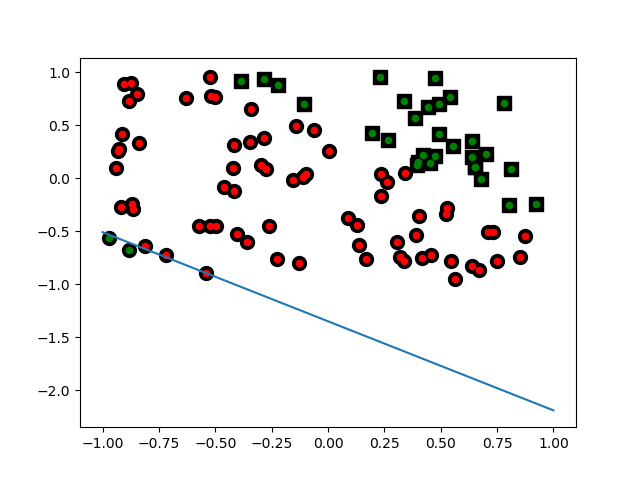
\includegraphics[width=10 cm]{Perc_before.png}
	\caption{classificazione prima del training}
	\label{fig:percBefore}
\end{figure}
Nella rappresentazione grafica (figura \ref{fig:percBefore} ) le due classi son rappresentate con quadrati e cerchi colorati di rosso o verde se sono classificati rispettivamnente in modo corretto o errato.
La funzione effettiva di classificazione è la retta di colore rosso, in blu è presente quella stimata (inizialmente con pesi random).\\
Il programma prosegue con dei cicli di training.
\begin{lstlisting}[language=myPython]
 trainCycle(population, perc, <?\color{magenta}{\textbf{5}}?> )
\end{lstlisting}
Per questo esempio il percettrone viene sottoposto a {\color{magenta}5} cicli di training.
\begin{lstlisting}[language=myPython]
 def <?\color{OliveGreen}{\textbf{TrainCycle}}?> (populationG, pa, number):
	for i in range(number):
		for i in range(50):
			dot = choice(population)
			pa.train(dot.pos, dot.group)
\end{lstlisting}
La funzione {\color{OliveGreen}{\textbf{TrainCycle}}} seleziona 50 elementi randomici (funzione choice in python estrae casualmente da una collezione ) su 100 e li usa come train set.
\newpage
\begin{lstlisting}[language=myPython]
 def train (self,inputs,target):
	guessed = self.guess(inputs)
	error = target-guessed
	for i in range(0,len(self.weights)):
		<?\textcolor{blue}{self.weights[i] += error*inputs[i]*self.lr}?>
\end{lstlisting}
La funzione di train del percettrone rivaluta i propri pesi secondo la formula:

$$\color{blue}\underline{w}=\underline{w}+\underline{err}*\underline{input}*learnRate$$

L'output ottenuto dopo i cicli di training mostra una classificazione corretta.
\begin{figure}[h!]
	\centering
	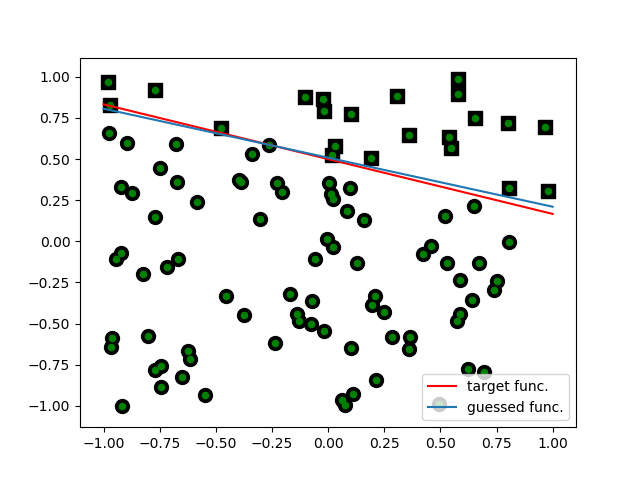
\includegraphics[width=10 cm]{Perc_after.png}
	\caption{classificazione dopo il training}
	\label{fig:percAfter}
\end{figure}
\newpage
%#######################################################################
\section{Doodle classifier}
Lo scopo del progetto è stato ottenere un classificatore in grado di distinguere con una buona precisione a cosa somigliasse di più un disegno rispetto a altri riferimenti passati in precedenza.\\
Nel caso specifico sono stati utilizzati tre dataset contenenti disegni di nuvole,uccelli e della torre eiffel.
\subsection{Neural network}
Il primo passo è stato creare una classe per la rete neurale dotata di un solo hidden layer (\textit{basic1NN/neuralNet.py}). 
\begin{lstlisting}[language=myPython]
 def __init__ (self, input_size,hidden_size,out_size):
	self.input = []
	self.iS = int(input_size)
	self.oS = int(out_size)	
	self.weightsI = np.random.random(( hidden_size,input_size))*2-1
	self.weightsO = np.random.random((out_size,hidden_size))*2-1
	self.bias_h = np.random.random((hidden_size,1))*2-1
	self.bias_o = np.random.random((out_size,1))*2-1
	self.lr = 0.1
	self.output = np.zeros(out_size)
\end{lstlisting}
\newpage
Sono state implementate successivamente le funzioni di feed forward e di backward propagation
\begin{lstlisting}[language=myPython]
# funzione di feedforward
def ff(self): 
	self.hidden = sigmoid(np.dot(self.weightsI,self.input)+self.bias_h)
	self.output = sigmoid(np.dot(self.weightsO,self.hidden)+self.bias_o)
\end{lstlisting}
Le operazioni effettuate sono rappresentati nella figura \ref{fig:hidden} e \ref{fig:output} escludendo la sigmoide usata come funzione di attivazione
\begin{figure}[h!]
	\centering
	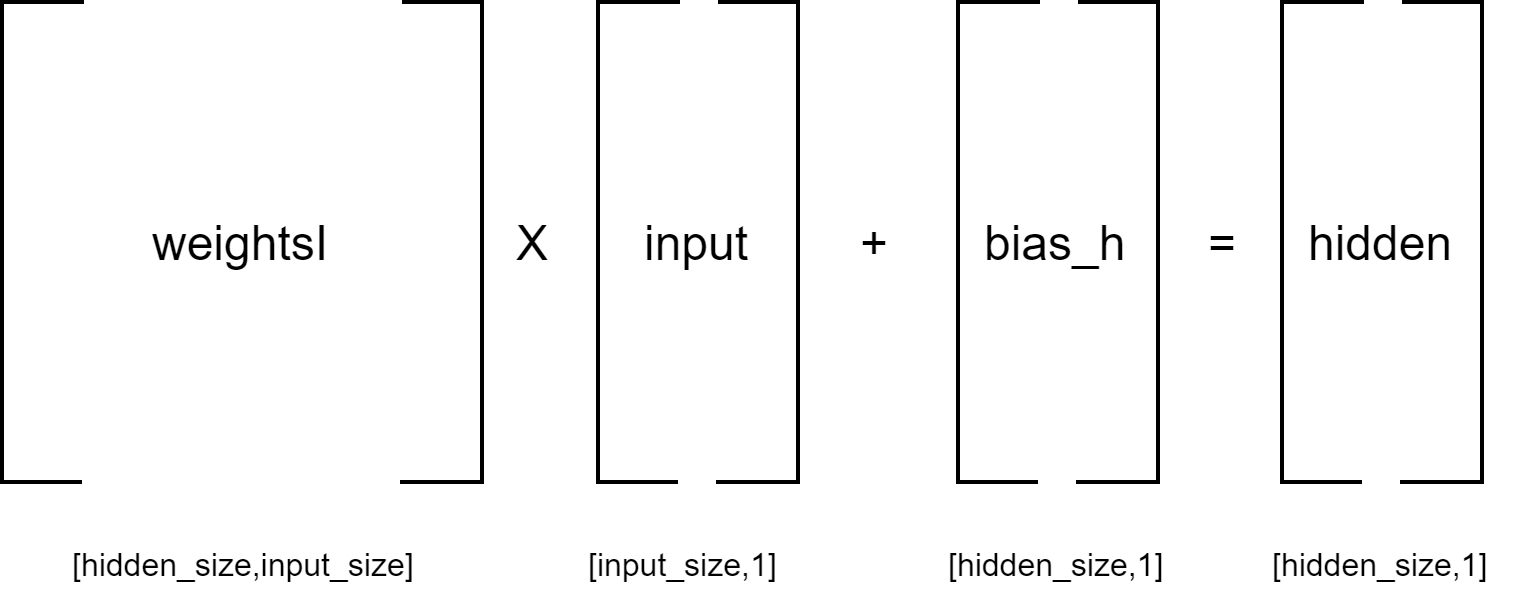
\includegraphics[width=10 cm]{resources/hidden.png}
	\caption{rappresentazione matriciale degli argomenti della classe usati nel calcolo dei valori dell'hidden layer}
	\label{fig:hidden}
\end{figure}
\begin{figure}[h!]
	\centering
	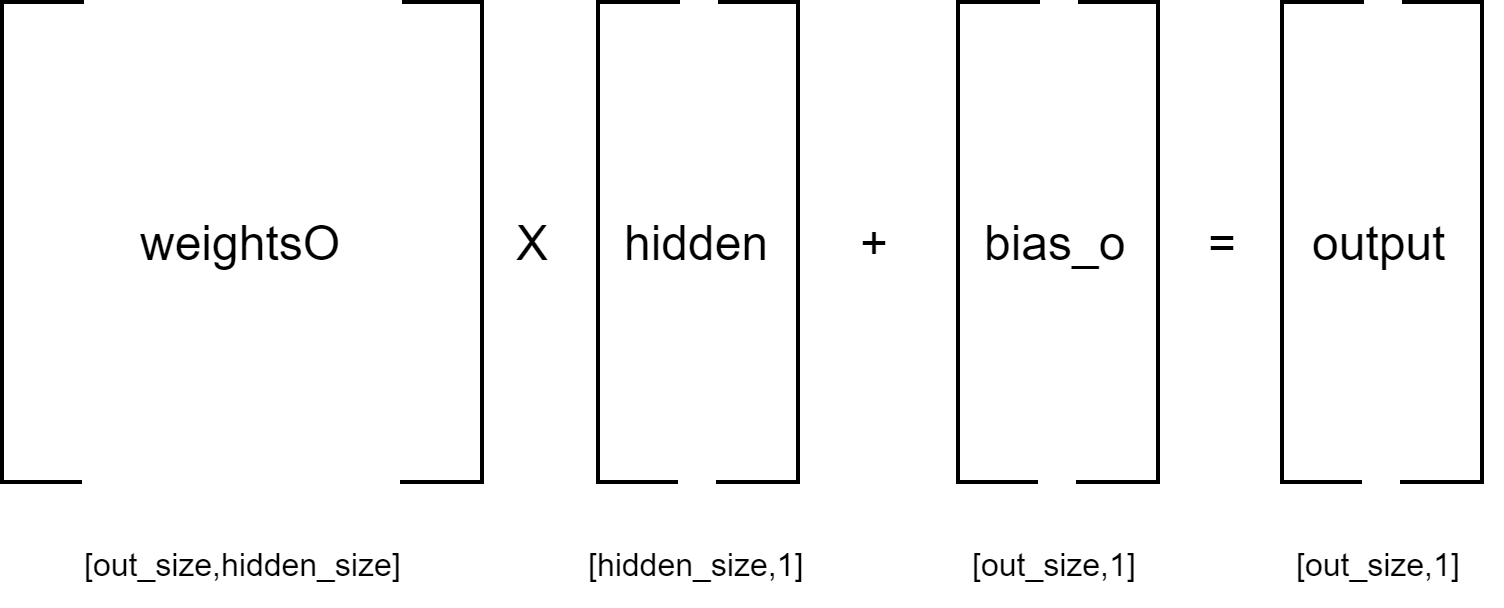
\includegraphics[width=10 cm]{resources/output.png}
	\caption{rappresentazione matriciale degli argomenti della classe usati nel calcolo dell'output}
	\label{fig:output}
\end{figure}
\newpage
\begin{lstlisting}[language=myPython]
# funzione di backward propagation
def backprop(self):
	out_err = self.y-self.output
	gradiente_o = (sigmoidD(self.output)*out_err)*self.lr
	delta_ho = np.dot(gradiente_o,self.hidden.T)
	self.weightsO+=delta_ho
	self.bias_o+=gradiente_o
	gradiente_h = sigmoidD(self.hidden)*np.dot(self.weightsO.T,out_err)*self.lr
	delta_ih = np.dot(gradiente_h , self.input.T)
	self.weightsI += delta_ih
	self.bias_h += gradiente_h
\end{lstlisting}
La funzione di backward utilizza la formula:
\[out\_err=target-output\]
\[ \nabla_o=({\sigma'(output)}*(out\_err))*learningRate \]
\[ \Delta_o=\nabla_o * hidden^T \]
\[weightsO= weightsO+\Delta_o\]
\[bias\_o=bias\_o+\nabla_o\]
\[ \nabla_h=({\sigma'(hidden)}*(weightsO^T*out\_err))*learningRate \]
\[\Delta_i=\nabla_h*input^T\]
\[weightsI=weightsI+\Delta_i\]
\[bias\_h=bias\_h+\nabla_h\]
Per velocizzare l'esecuzione del codice sono state inserite delle funzioni per importare/esportare ( importPar(),export() ) i pesi (weightsI,weightsO,bias\_h,bias\_o)in modo da non dover fare training ogni volta prima di eseguire il codice.
\newpage
\subsection{Main file}
Nel file principale ( \textit{./googleDoodle.py} ) se la rete neurale non fosse gia pronta si puo impostare la variabile TRAIN per inizializzare il dataset e eseguire le funzioni di train.
\subsubsection{Training}
Viene effettuato il training su 3 differenti dataset di disegni. Le immagini sono 28x28 pixel e sono salvati in file di numpy (libreria di python).
\begin{lstlisting}[language=myPython]
if TRAIN:
	clouds=np.load("dataset/cloud.npy")
	...
	splitClouds=int(120265*0.75)
	TrainClouds,TestClouds = np.split(clouds,[splitClouds])
	...
\end{lstlisting}
Il dataset delle nuvole ad esempio viene caricato e diviso al 75\% (120265 è il numero totale di samples nel dataset delle nuvole) in due per il training e testing rispettivamente.
\begin{lstlisting}[language=myPython]
import basic1LNN.neuralNet as nn
oracle = nn.NeuralNet(784,64,3)
\end{lstlisting}
Viene creata una rete neurale con un input di 784 (pixel totali dell'immagine),64 nodi nell'hidden layer e un output di 3 ( per i 3 dataset utilizzati).
\newpage
\begin{lstlisting}[language=myPython]
if TRAIN:
	trainingSet = []
	print("generating training set")
	for i in range(splitBirds-1):
		x=np.reshape(TrainBirds[i]/255.0,(784,1))
		y=np.reshape(np.array([1,0,0]),(3,1))
		trainingSet.append([x,y])
	for i in range(splitClouds-1):
		x=np.reshape(TrainClouds[i]/255.0,(784,1))
		y=np.reshape(np.array([0,1,0]),(3,1))
		trainingSet.append([x,y])
	for i in range(splitEiffel-1):
		x=np.reshape(TrainEiffel[i]/255.0,(784,1))
		y=np.reshape(np.array([0,0,1]),(3,1))
		trainingSet.append([x,y])
	r = random.SystemRandom()
	r.shuffle(trainingSet)
	for el in trainingSet:
		oracle.trainOnce(el[0],el[1])
	oracle.export()
else:
	oracle.importPar()
\end{lstlisting}
Le immagini del train set vengono quindi prese singolarmente, convertite in vettori con valori da 0 a 1, associati alla terna corrispondente all'immagine (e.g. 0,1,0 per i disegni di nuvole) e inseriti in un database unico che verrà poi mescolato per avere un training uniforme.
\newpage
\subsubsection{Guessing}
Il programma prende in input il file myInput.png posizionato nella stessa cartella di \textit{googleDoodle.py}, lo converte in un formato compatibile e tramite il metodo answer() della classe NeuralNetwork ottiene la classificazione.
\begin{figure}[h!]
	\centering
	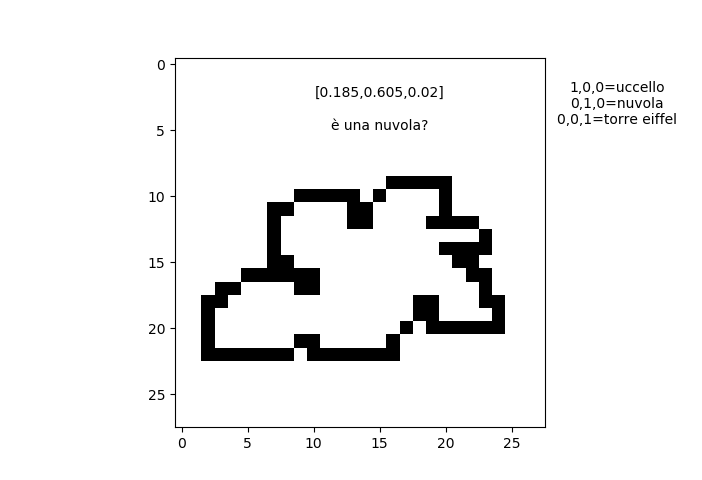
\includegraphics[width=15 cm]{output.png}
	\caption{output post esecuzione}
	\label{fig:procOutput}
\end{figure}
\newpage
\begin{thebibliography}{9}
\bibitem{googleDoodleProject}
Dataset di google:\\
https://github.com/googlecreativelab/quickdraw-dataset 
\end{thebibliography}
\end{document}